\documentclass[a4paper, 10pt, english]{article}
%\documentclass[a4paper, 10pt, swedish]{article}

\usepackage[T1]{fontenc}        % Allow for åäö
\usepackage{lmodern}            % Better font for åäö
\usepackage[utf8]{inputenc}     % For åäö in text


\usepackage{babel}              % Language specifics
                                % + hyphenation

\usepackage{subfigure}
\usepackage{amsmath, amssymb}   % Math stuff
\usepackage{gensymb}

\usepackage{graphicx}           % For including graphics
\usepackage{epstopdf}
\bibliographystyle{plain}       % References
%\bibliographystyle{sweplain}    % Swedish references

\usepackage{textcomp} 

\usepackage[margin=1in]{geometry}


\usepackage[colorinlistoftodos]{todonotes}					% Todo notes

\usepackage{tikz,pgfplots} 
\pgfplotsset{compat=newest} 
\pgfplotsset{plot coordinates/math parser=false} 

\usepackage{fancyvrb}

\newcommand{\transp}{^\mathsf{T}}
\newlength\figureheight 
\newlength\figurewidth 


\title{WASP SECC Course: Cloud Module Assignment\\Architecture}
\author{Kristoffer Bergman, Per Boström, Shervin Parvini Ahmadi}
\date{May, 2017}


\begin{document}
\maketitle

\section{Overview}

\begin{figure}
	\label{fig:architecture}
	\centering
	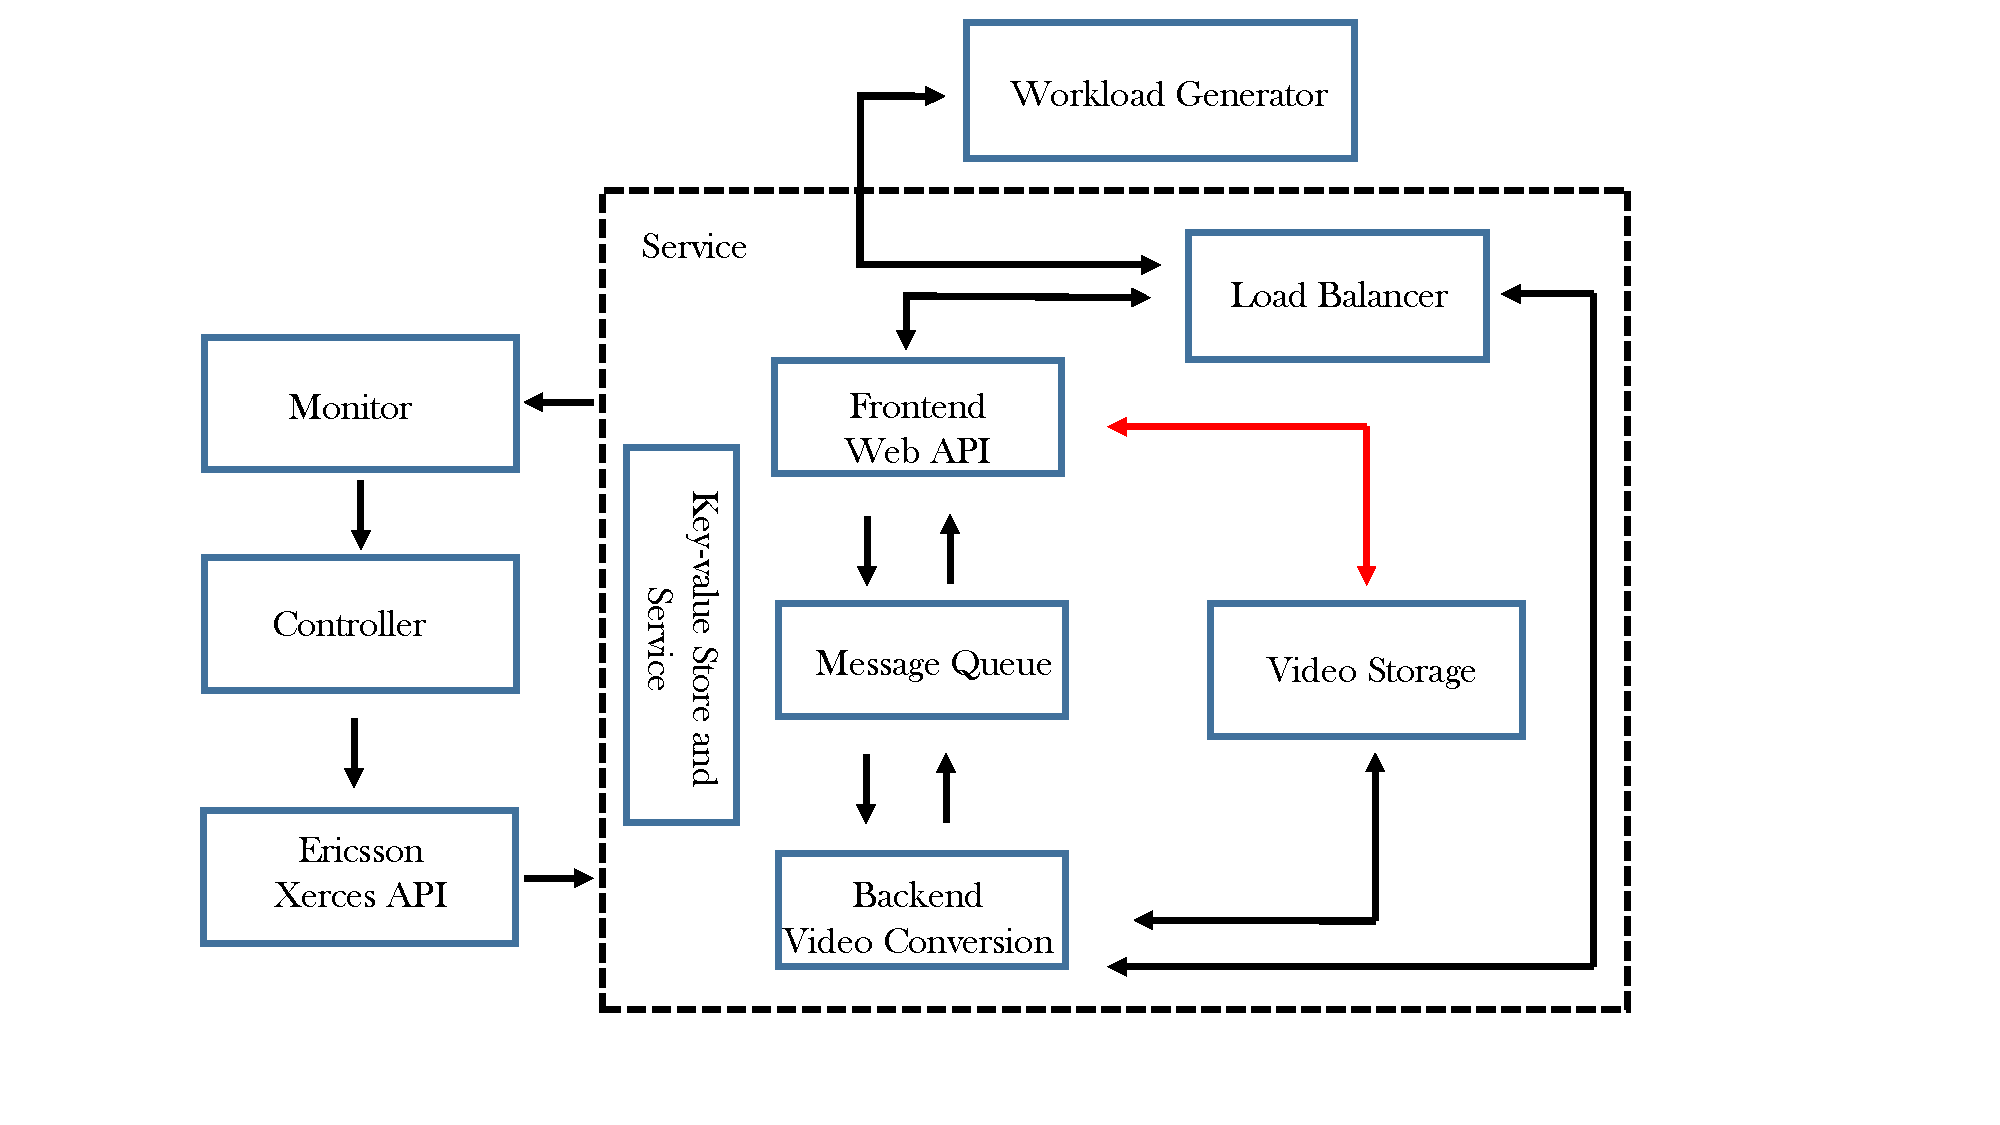
\includegraphics[width=1\textwidth]{figs/workflow.pdf}
	\caption{Overview of the architecture.}
\end{figure}
An overview of the proposed architecture can be found in Figure~\ref{fig:architecture}. The different components involved are:
\begin{itemize}
	\item \textbf{Workload generator}: Will be used as a test engine to simulate external users. See Section~\ref{sec:WG} for more details.
	\item \textbf{Load balancer}: Will be used to distribute the workload across the multiple instances of the frontend Web API. It will also be used for the backend Video conversion, but we are currently not completely sure on how to use this component. 
	\item \textbf{Frontend Web API}: Will be used to receive requests from users and deliver a response. We have simplified the architecture so that we only acknowledge the user when the conversion is completed and how it should be related to the controller specified in Section~\ref{sec:Controller}.
	\item \textbf{Message queue}: Will be used to route the requests to the available Video conversion nodes and maintain the request queue. Will also route the responses after video conversions.
	\item \textbf{Backend Video conversion}: Will be used to do the actual conversion of videos by reading the video from the storage.
	\item \textbf{Video Storage}: To simplify the assignment, we will use a storage node that contains all the available videos for conversion. To simplify things further, we are considering not to send the converted video to the user. Instead, when the conversion is complete, the converted video will be deleted (and the user notified that the conversion is completed).
	\item \textbf{Monitor}: Will be used to monitor entities relevant for the controller, by periodically gather information. It will also save this information in .mat files, which can then be used to plot the data in Matlab. 
	\item \textbf{Controller}: Will be used to make the service scalable. See Section~\ref{sec:Controller} for more details.
	\item \textbf{Key-value Store and Service}: Will be used to perform health checking for the service as a whole.	
\end{itemize}

\section{Software and tech}
The following is a list of the software and tech that will be used to implement the system components:
\begin{itemize}
	\item \textbf{Workload generator}: Python code and REST
	\item \textbf{Load balancer}: nginx
	\item \textbf{Frontend Web API}: Python
	\item \textbf{Message queue}: RabbitMQ
	\item \textbf{Backend Video conversion}: Mencoder
	\item \textbf{Video Storage}: Object storage in OpenStack? 4k Video Samples will be used for gathering videos to be placed in the storage.
	\item \textbf{Monitor}: Python
	\item \textbf{Controller}: Python and Python novaclient (For interacting with OpenStack to start or kill VMs). 
	\item \textbf{Key-value Store and Service}: etcd
\end{itemize}

\section{Redundancy}
To increase the robustness of the system, we will use redundancy for the following components:
\begin{itemize}
	\item Message Queue
	\item Load Balancer
	\item Key-value Store and Service
	\item Monitor
\end{itemize}
By redundancy, we mean that we will use one (or more) backup components that contains the same data as the main component. In case of failure, the backup component takes over.
\section{Workload generator} \label{sec:WG}
The workload generator is the test engine that simulates external users. It takes two parameters: the number of client converters and the average time between conversion requests. It will start the specified number of client threads of which each one represents a user. Each client randomly selects a video, sends a conversion request, waits for the completion, and then sleeps for a while (on average the specified time) before repeating the process.

The workload generator will also measure values such as response time and keep track of how many requests there are in the queue.
\section{Controller} \label{sec:Controller}
In order to make the service scalable, we must be able to scale up or down depending on its load. For this, we need a controller that controls the number of nodes used to convert videos (backend) and also nodes that receives conversion requests (frontend). The scaling will be performed horizontally.

We will use the simplifying assumption that all videos are of approximately the same size. This makes it possible to use the time from that a video conversion request is submitted until the video is converted as the control objective. Assume the average time it takes for one core to convert one video is given (including potential delays in the system), and denote it $ T_{\text{conv}} $. With $ n_{\text{queue}} $ video conversion requests in queue and $ n_{\text{vm}} $ active VMs, the time $ T $ needed to convert all videos in the queue is given by
\begin{equation}
T = \frac{T_{\text{conv}}  n_{\text{queue}}}{n_{\text{vm}}}
\end{equation}
Thus, if the control objective is to keep the maximum time from a request is submitted until the video is converted below $ T_{\text{max}} $, the number of VMs needed is given by
\begin{equation}
n_{\text{vm}} > \frac{T_{\text{conv}}  n_{\text{queue}}}{T_{\text{max}}}
\end{equation}

This is of course a simple approach which, if needed, could be extended to also consider videos of varying sizes and possibly reordering the queue such that for example small sized videos are prioritized over larger ones.

\subsection{Oversubscription}
Due to oversubscription, the provided cloud environment does not guarantee that adding one VM will lead to an overall increase in performance, nor that all VMs will have the same performance over time. Assuming conversion rate in Mb/s, \emph{i.e.} an entity inverse proportional to the time needed to process a video, depends on the number of active VMs in a way similar to Figure~\ref{fig:vmvsMbs}, it should be possible to optimize the number of VMs, to avoid wasting resources.
\begin{figure}
	\label{fig:vmvsMbs}
	\centering
	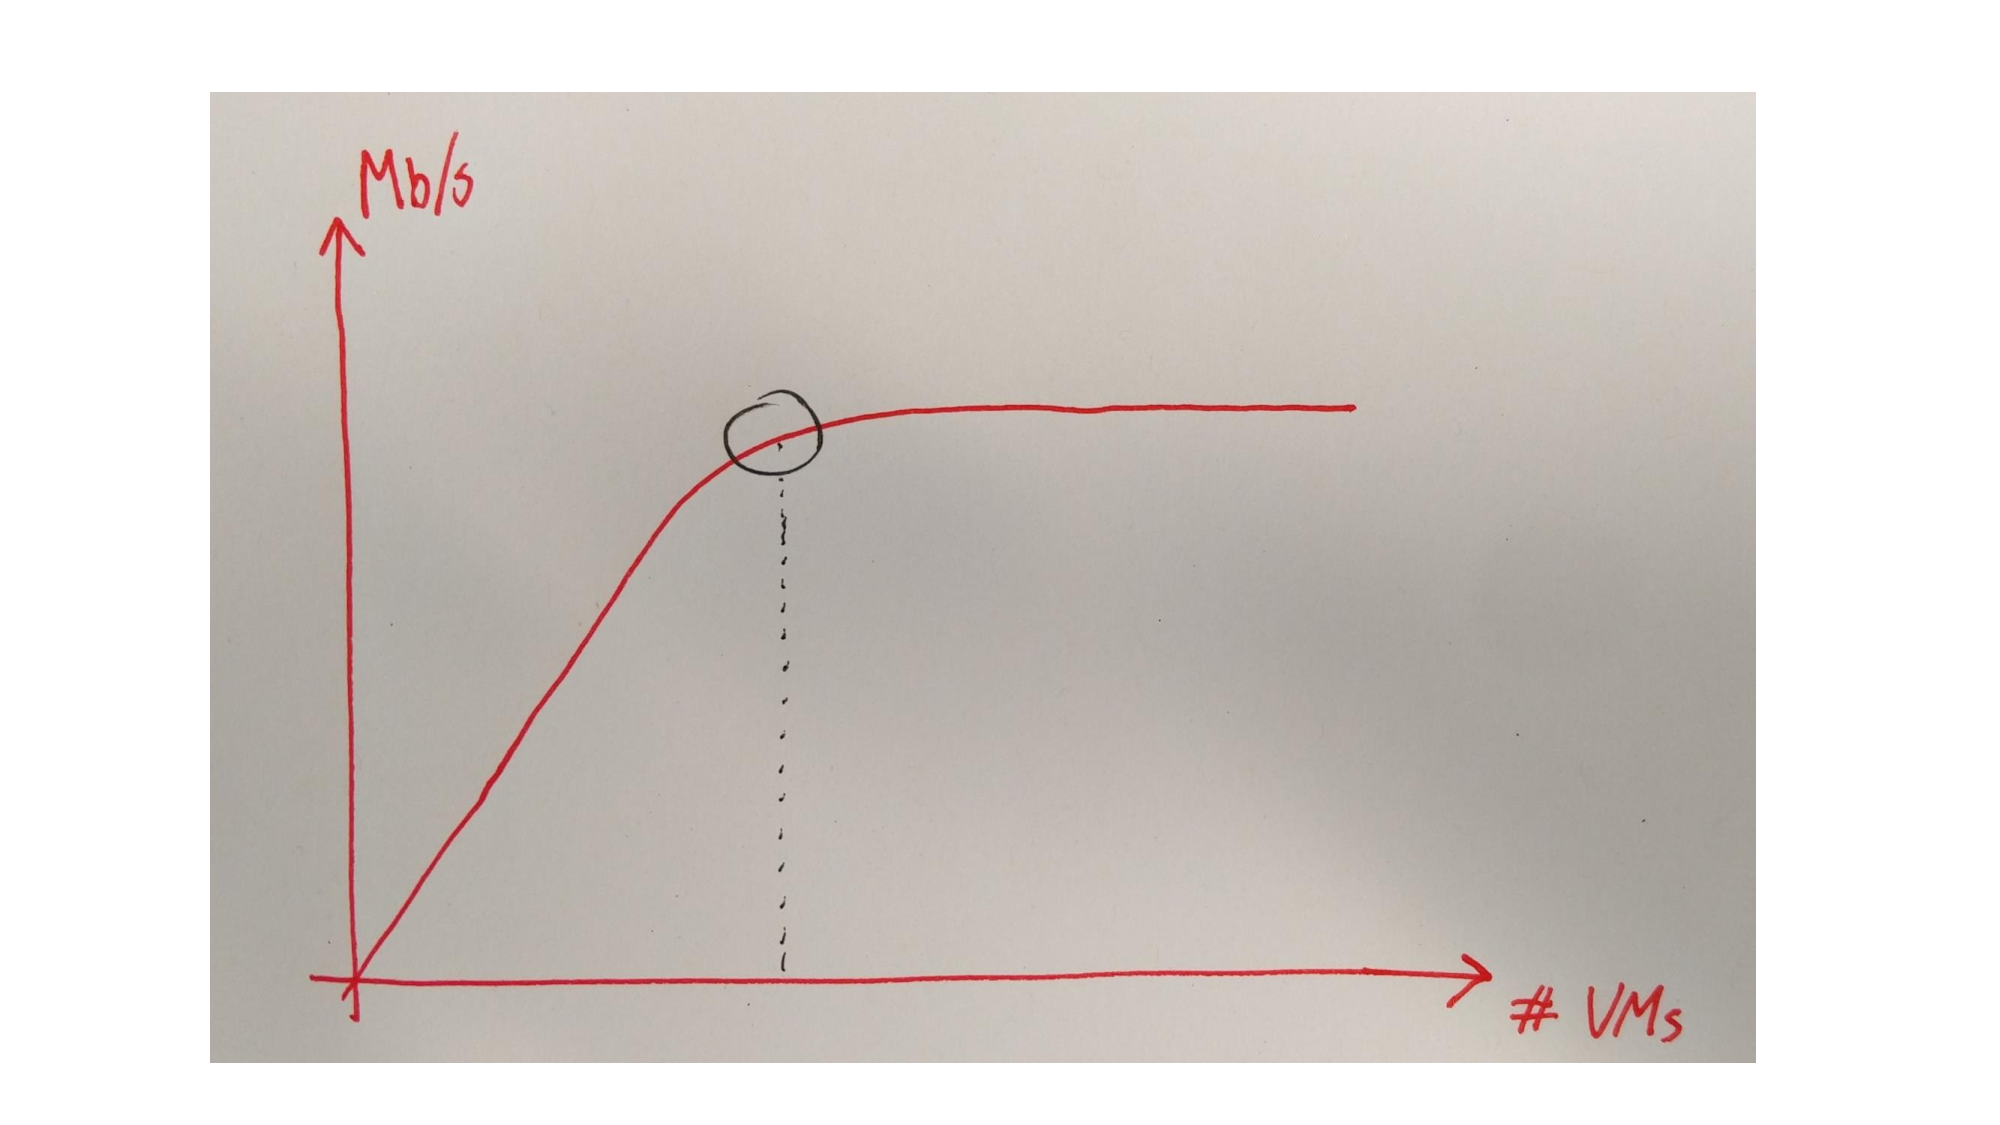
\includegraphics[width=.6\textwidth]{figs/vmvsMbs.pdf}
	\caption{Assumed behavior of the video conversion rate as a function of active VMs. There is no gain in conversion rate if more VMs are added passed the circle.}
\end{figure}

\end{document}